\documentclass[a4paper,12pt]{article}
\usepackage{graphicx}
\graphicspath{{images/}}

\begin{document}
\title{Software Requirements Specification for WitsCABS\\Lab 2 Submission - Group 10}\author{1171733 - Jason Stuart (GL), 669006 - Rashad Akoodie, \\1064934 - Robert Basson and 886515 - Amine Boukrout}
\date{\today}
\maketitle
\newpage
\tableofcontents
\newpage

\section{Introduction}
\subsection{Purpose}
The purpose of this document is to describe what is required for the development of WITSCABS (a lift service similar to the one provided by Uber). This document is meant to convey how we have decided to develop our system and the functionality required for the first release. This will be achieved through a description of the scope of the software being designed, so that the project bounds are clearly defined, in order to prevent scope creep. The document will then for both the front and back ends describe their functional requirements.There will also be a description of the software required to be integrated with our software solution in order for it to be functional according to the requirements. 
In addition to this, a fully descriptive documentation of all programming techniques as well as software engineering techniques that we as a group will follow during development will be included. These techniques will be substantiated in order to provide a clear systematic approach to the complete design of our project. Furthermore, all resources consulted will be included as well.
\subsection{Problem Statement}
WITS students often require transport to get them from place to place, it could be to and from a place of residence, shopping centers, places to support wits sports, internet cafes etc. Wits would like to implement a transport system similar to Uber that Wits students are able to use as a means of travel.

\subsection{Scope}
Our core objective is to design, develop and implement a software system which will be used to manage a fleet of taxi-cabs for a company (as per the project brief). Our company, “WitsCABS Company”, will be independently run and will employ our own staff/drivers. Vehicles however may either be owned by WitsCABS Company or by the drivers. The service will run based on “service zones” within the city of operation i.e. the city will be split into various sectors which will allow for more efficient ride time. Each driver will be equipped with a smart-phone embedded with GPS, maps and a navigational tracking system. All vehicles being dispatched will be on instruction from the 24-hour manned Dispatching Control Centre (DCC) which will be in direct contact with clients via calls to the centre.
\\\\
The front-end of our system will comprise mainly of an android application used by the drivers which will be integrated with a GPS and mapping service such as Google maps to optimize routes taken as well as save time in the case of human error. A simple website will be set up as well to deal with customer queries/complaints and basic information about WitsCABS. To achieve this, we will be primarily using Java as a programming language as well as some HTML and Javascript. The front-end of our mobile android application will consist of the visual representation of the map being used as well as any turning signals or warning, messages etc. needing to be displayed on the screen, a login screen for the drivers where they would enter their credentials, a waiting screen for when they are awaiting a client. Furthermore, the drivers should communicate with the DCC. For this, a web-based application and/or application will need to be created for the DCC where they can view the entire city of operations. The front-end of this “application” would comprise of a form that will allow the DCC to capture customer details. It will then send these details to the back-end which will then determine which cab to assign.\\ \\
The Back-end of our system will make use of Java as well as JSON. This will consist of storing all the driver’s information (Names, license number, car registration, age etc.) as well as each trip he works as well as any necessary information about the passenger transported. It will also be integral to integrate the maps into finding which driver is best suited for the next pickup requested based on some sort of efficiency algorithm which we will design. This information would most probably need to be stored in a database and communicate with our mobile application using JSON. Another useful system to have would be to record every client that has rode with one of our cabs before and perhaps assign a customer number or ID to use the following time he/she requests a ride. \\\\
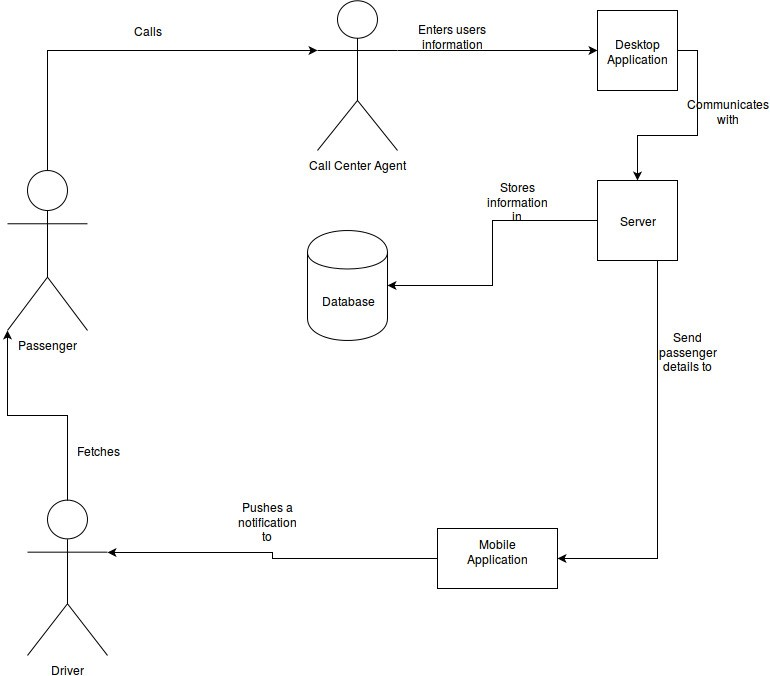
\includegraphics[scale=0.8]{user_flow}
\pagebreak
\subsection{Overview}
The document will be broken up into multiple sections. As already mentioned before in the document, we have given an introduction as to why this document has been typed up, as well as a scope of what the project is all about and a basic description of the required features needed to be implemented.\\\\ In section 2, an analysis of how the project will be conducted is discussed. This includes a discussion of system architecture types, software required for the project, as well as how the team will be managed and handled during development. \\\\In section 3, a list of formal required functions will be provided for both front-end software as well as the back-end.
\pagebreak
\section{Analysis}
\subsection{Team Administration}
\subsubsection{Team Management}
Our team has decided to take the Agile SCRUM method as our SDLC (software development life cycle). We chose this approach based on multiple reasons. Due to the short time constraint given to us by the client, a rapid development approach is needed, one that is satisfied by Agile development.\\\\ We also require quite a bit of feedback from the client, hence this iterative approach is best as it allows us to be in constant communication with the client, with small changes in between, allowing us to quickly change anything the client is unhappy with. Another advantage of SCRUM specifically, is that we will constantly be meeting up each day either in person, or by Google Hangouts to check up on the group and what each member has done over the last day, allowing us to keep a high morale and high sense of worth in the team, even though the time requirement is strictly short. Since our team is highly motivated already and have experience in development, they can be trusted to handle their tasks efficiently, another benefit of the SCRUM process, where each developer has more responsibility than in other methodologies. Also, since our team is relatively small, SCRUM will also work, as there will not be as much time required to structure and organize the team as a whole, increasing productivity. Also, since SCRUM focuses more on the actual development and less on the documentation, since we are going to be showing each change to the client, it benefits the productivity even more.
\\\\We have also considered the disadvantages of SCRUM. We understand that there is a higher chance of Scope creep with Scrum, but this is why we have already defined the scope of the project in the beginning of this document, to define clear boundaries to the project, to prevent this from happening. We have also been very clear with our functional requirements needed for a successful project, to prevent inaccurate measurement of time estimations.\\\\ Furthermore, SCRUM has the possibility of failure, if at least 1 member loses interest or focus. This is why we have nominated a clear leader to take charge and to keep the team motivated, regardless of what may come. If a team member were to leave, this would also have a large inverse effect on the project, however this will not happen, as each member is fully committed to this project, as this project results in marks required to graduate. \\\\Finally, it may be hard to quantify quality as the software is rapidly evolving, however since we do not have a quality control team, we can work on quality between each developer to keep the project from slipping quality wise.
\subsubsection{Team Meetings}
The team will conduct the project as follows:
\begin{itemize}
\setlength\itemsep{0em}
\item [] Each team member will be required to be at each sprint planning meeting every 2 weeks, from the start of the project. This meeting will be organized by the Group Leader, i.e. the scrum master.
\item [] Each member will be required to be available for the daily stand up meeting, preferably in person, otherwise via Google Hangouts. Each member should be able to describe to the team what they have worked on over the past 24 hours. Thereafter each member will describe what they will work on for the next 24 hours. 
\item [] The scrum master will ensure that the project is moving at a reasonable pase and that all team members are motivated at all times.
\end{itemize}
\subsubsection{Responsibilities of Team}
Our current student assignment is as follows. Rashad and Amine will handle the mobile app. Robert will handle the frontend. Jason will handle the backend. As the project moves forward, this can change, depending on who needs what help at each time. Each member is responsible for providing constant communication and feedback on their portions as well as suggestions on others work. Jason will schedule any meetings required to advance the project in any way.
\subsection{System Architecture Analysis}
After thorough analysis of existing architectures and analyzing the functional requirements listed later in this document, the team has decided to make use of a 2 part Client - 1 part Server architecture. The first client software will be the mobile app that allows the drivers of the WITSCABS service to receive communication from the system as to who the driver should pick up, etc. \\\\The other client software will be run on a desktop in the call center, so that as a client calls in, the operator can input all the details necessary for the system to compute the best driver to use. The server will be the bridge between these two client software services, where the server determines the best driver for the job that arrives and pushes the required information through to the driver on his mobile app.\\\\ All this communication will be facilitated through an Internet connection, so when designing the system, it must take into consideration that an internet connection might not always be available for the drivers. There is no need to have any further server or client interfaces thereafter.
\subsection{Analysis of Front-end System (Mobile App)}
We have decided to make use of an android application as the primary user-accessible interface for our project. The reason for choosing a mobile application is quite obvious in our case as the drivers who will be using the application have to be in their vehicle at the time of using the application as well as moving in the vehicle while using it. This automatically squashes any idea of a desktop application or web based application as the accessibility would be a major issue. The possible downside to this would be that each driver requires a cellphone/tablet which will support the software WITSCabs as well as a mobile data connection. \\\\
The call centre will be using a desktop application in conjunction with the android application although the users will not be registered to the database but instead will have access to the database in a read-only capacity. This will allow the call-centre to access client details as well as driver’s details which will in turn allow them to run statistics checks as well as be prepared in the case of an emergency. For this, it is clearly most beneficial to use a desktop application preferably with an internet connection as immediate run-time statistics as well as driver locations etc. are imperative.\\\\
For this purpose we have chosen to develop our software as an android application as it is the most common operating system friendly platform for a mobile application. Linking with this, it has been decided as a group that a predominant bulk of the code used should be Java as it is the most commonly used programming language for Android applications as well as the most familiar between each member of the group. Adding to this, we have decided to use IntelliJ idea as an IDE for our app development as it is popular, free to students and boasts many high-end features which will benefit the development of our project.
\subsection{Analysis of Front-End System (Desktop App)}
When a user wants to get a lift they have to call in and speak to a call center agent. The call center agent will then get the relevant information from the user and capture it in a desktop application. This application will communicate with a server which will capture the information in a database. The server then sends a notification to the mobile application so that a driver can pick up the user.\\\\
We have chosen to use a desktop application over a web application. The main reason for this is responsiveness. Web applications can become unresponsive if the internet connection is heavily used or if there are connectivity issues such as a damaged line, desktop applications have a more reliable response time as response time will be limited by the CPU. Desktop applications are also more secure than web applications which will be important as we store user information on a database.\\\\
The language chosen to develop the desktop app is Java. Java is platform independent so it will run no matter what operating system is on the call center computers. Java is an easy to learn object oriented language, this helps us to create reusable code. Another benefit of Java being easy to learn is its popularity, this means that should any problems arise it won't be difficult to find someone to fix these problems.
\subsection{Analysis of Back-End System}
The back-end will consist of two parts. The server application and the database.
Our database will be developed using the DBMS MySQL. MySQL is a very commonly used and simple DBMS so any issues with the database can be dealt with quickly and easily. As MySQL is very easy it only requires basic statements in order to interact with the database. We have also chosen MySQL as it is free which helps reduce the cost needed to develop the full system. MySQL is also able to handle large amounts of data which is well suited for a popular application. The DBMS also includes options to add security which can help protect the data in the database from intruders.
\\\\
The development of the back-end is important even though the user does not interact with it. We need a means to store user information and assign drivers. This back-end actually serves as the lifeline for the system. Hence this will also be developed with Java, since all the members of the team are most familiar with the language and how to implement networking to the highest efficiency possible.
\subsection{Additional Software API’s Required}
Due to the nature of the project, the implementation of the software application will require external software and most probably certain add-ons from the supporting software. One of the main supporting software that is required to actually implement the application is Google maps along with its various API’s. This is required since the application has to be integrate with Google maps in order to provide a GPS service to guide the driver to the location of the customer. \\\\
A type of a database management system (DBMS) will be required in order to keep relevant information about the operations of the business. Such information would include login details, customer details, driver details, trip details, etc. Most probably the DBMS that will be used is either MySQL or PostgreSQL. It is worthwhile to note that as the project progresses additional software requirements may arise, and in this regard the client will be notified.

\subsection{Analysis of Inputs and Outputs}
\subsubsection{Inputs}
The first type of input would be a phone call from a customer providing information such as the pickup location, customer name, and contact number. The dispatching control center (DCC) agent will enter the information provided by the customer into a database by using an interface that will run on a localised desktop at the DCC. Once the information is stored on the database, the system will allocate a customer to a driver based on whether or not a driver is available or not (by using an algorithm designed and agreed upon by the developers). The driver will then be provided with the GPS information of the customer which will be inputted into the embedded GPS on the driver's smartphone.

\subsubsection{Outputs}
Once the driver has been allocated, a notification will be sent firstly to the driver via the designed app to notify him/her about the customer?s assignment to that particular driver and basic information, such as the customer?s name and contact number, along with the physical address or GPS coordinates that the customer provided (this can be displayed the driver?s app as link which could launch the designed application for the company or the GPS app embedded in the smart phone). On the customer?s side, he/she will receive a SMS when the driver is in a predefined range from the address provided by the customer.

\pagebreak
\section{Functional Requirements}
\subsection{Front-End Mobile App}
\begin{description}
\setlength\itemsep{0em}
\item Send Status updates to the server on whether this driver is available or not
\item Send location updates so the server knows where you are when status is marked available.
\item Be able to receive passenger information that will help the driver find the passenger.
\item Find the quickest route to the destination.
\item Update Driver details
\item Register Driver onto the system.
\end{description}
\subsection{Front-End Desktop Application}
\begin{description}
\setlength\itemsep{0em}
\item Create new passenger
\item Insert passenger into database via the server
\item Edit record
\item Push and save information to database
\end{description}
\subsection{Back-End Server}
\begin{description}
\setlength\itemsep{0em}
\item Accept incoming connections from desktop applications, which contains details related to the passenger in need of transport.
\item Analyze which service zone the passenger is located in.
\item Run an algorithm to find the closest driver ready to pick up a passenger
\item Send a push message to this specific driver with the details of the passenger to fetch as well as their destination.
\item Allow drivers to mark if available or not via a status change
\item Be notified when a driver is close to pick up point via SMS.
\item Be notified when passenger is there at their destination, to automatically mark drivers as complete, i.e. the driver is transitioning back to their house or service taxi rank. Thereafter the driver can mark they are ready for another job.
\end{description}
\pagebreak

\section{Evaluation}
\subsection{Compiling And Running Code}
\subsubsection{Desktop Application}
The Desktop Application to be used in the call center will be a Java program (as previously mentioned). So in order to compile it an IDE that supports Java will be required eg Eclipse or Netbeans. For the sake of this document it is assumed that Netbeans will be used. Further it is required that you have the latest JDK and JRE software installed from Oracle.\\
Netbeans has a built in compiler that is easy to use. On the ribbon at the top of screen there are two hammers, one hammer has a brush. These hammers are used to call ``build'' and ``clean and build''. Clicking either one of them will compile the code. The difference between the two is that clean and build completely recompiles the code, deleting former versions.\\
After compiling a .jar file should be present in the build folder of the Java project. This .jar  file can be transferred to computers in the call center and will allow the application to run without the need for an IDE.It will require the use of the command prompt.\\To run the code using an IDE there are multiple options, you can right click the main class and select run file, or click the green play button in the top ribbon. Either of these options will run the code if the code has been compiled or compile and then run the code. To run from the command line without the IDE installed, navigate to the file in the command prompt and then type: java -jar CallCenter.jar

\subsubsection{Server}
Similarly to the Call Center Desktop Application, the server has also been constructed using Java as the programming language in order to more easily maintain compatibility with all the other programs. So in order to compile the code, you can follow a similar approach to 4.1.1 for the desktop application. Note it is required that you have installed the latest java JDK as well as JRE software. There is however an extra step required to setup the database. One needs to install mySQL and install it to the system using the default settings. When setting up user details, set the root password to ``jason''. Keep the port number the default. Furthermore, make sure to restore the current database from the repository code to the server using mysql -u root -p WitsCABS < WitsCABS.sql where this command is run in the same directory as the sql backup. Finally, to make sure that you can receive connections from client programs, make sure to give them your current ip address to input into their programs. 
To run the database, follow the similar setup as for the desktop application, i.e. navigate to the .jar file in the command prompt and then type: java -jar WitsCABS\_Backend.jar


\pagebreak
\section{Credentials}
\subsection{The Credentials}
\begin{description}
\setlength\itemsep{0em}
\item Purpose by Robert, Rashad, and Jason (Section 1.1)
\item Problem Statement by Robert (Section 1.2)
\item Scope by Amine (Section 1.3)
\item Image Process Diagram by Robert
\item Overview by Jason (Section 1.4)
\item Team Management by Jason (Section 2.1.1)
\item Team Meetings by Jason (Section 2.1.2)
\item System Architecture Analysis by Jason (Section 2.2)
\item Analysis of Front-end System (Mobile App) by Rashad (Section 2.3)
\item Analysis of Front-End System (Desktop App) by Robert (Section 2.4)
\item Analysis of Back-End System by Robert (Section 2.5)
\item Additional Software API’s Required by Amine (Section 2.6)
\item Analysis of Inputs and outputs by whole team (Section 2.7)
\end{description}
\subsection{Task and Responsibilities Dedications}
\begin{description}
\setlength\itemsep{0em}
\item Front-End Mobile App to be handled by Amine and Rashad (Section 3.1)
\item Front-End Desktop Application to be handled by Robert (Section 3.2)
\item Back-End Server to be handled by Jason (Section 3.3)
\end{description}
\end{document}